%Compare to phones!
Compared to smartphones one of the biggest advantages of Google Glass is the fact that Google Glass is a HMD. With a smartphone the user needs to either hold the smartphone in either one or both hands, alternatively put the smartphone on a table or the like. In other words can Google GLass offer a hands-free experience that smartphones can not.

Another advantage of Google Glass compared to smartphones is also due to the fact that Google Glass is a HMD. The user does not have to look away in order to see what is currently being displayed. Google Glass does not distract from what the user is currently doing as much as a smartphone where the user needs to either look away or hold up the smartphone in from of the eyes.

However, smartphones does give the user a bit more control. The control comes from the fact that smartphones supports multi-touch, which Google Glass does not. On a smartphone users may also touch on the screen, in contrast to Google Glass where the touchpad sits on the right hand side of the user. Google does, however, point out that Google Glass is meant to handle information that is simple.\cite{glassDesignPrinciples}

The smartphone screen size has been increasing ever since the iPhone first launched in 2007, as seen in Figure \ref{smartphoneSizeChart2}. Looking at currently available smartphones in Figure \ref{smartphoneSizeChart}, the increase in screen size does not seem to stop as the average screen size is approaching five inches. In terms of comparison to Google Glass the increase in screen size entails that more information could be displayed on a smartphone than on Google Glass.

Potentially the screen size of Google Glass will increase over time as well. However, one of the biggest difference between smartphones and Google Glass is the plural. Smartphone\textbf{s}. There are several smartphone brands competing on the market, each offering several models. Google Glass is simply Google Glass. As seen in section \ref{subsec:similarproducts} Google Glass does face competition that have approached HMDs differently, and as HMDs increase in popularity there is potential for an even wider offering of models and screen sizes.

%\url{https://developer.android.com/design/index.html}\\
%\url{https://developer.android.com/design/get-started/principles.html}
	\begin{figure}[ht!]
		\centering
		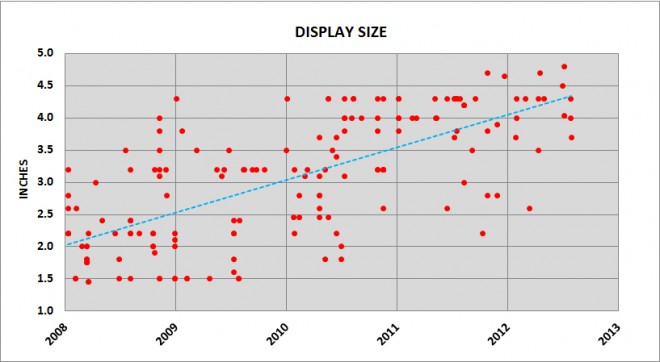
\includegraphics[width=110mm]{images/smartphoneSize2}
		\caption{Smartphone screens have been increasing ever since the iPhone launched in 2007.\cite{smartphoneSizeChart2}}
		\label{smartphoneSizeChart2}
	\end{figure}
	%http://www.pcworld.com/article/2455169/why-smartphone-screens-are-getting-bigger-specs-reveal-a-surprising-story.html

\hfill

%\url{https://developer.android.com/design/index.html}\\
%\url{https://developer.android.com/design/get-started/principles.html}
	\begin{figure}[ht!]
		\centering
		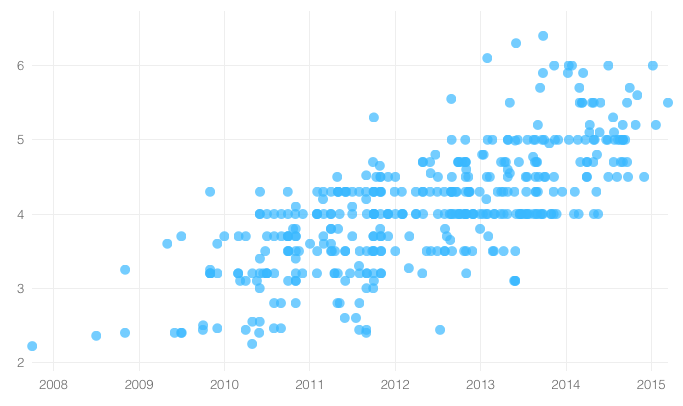
\includegraphics[width=110mm]{images/smartphoneSize}
		\caption{Smartphone screen sizes of the most popular of the currently available smartphones, where the x-axis shows the release date and the y-axis shows the screen size in inches.\cite{smartphoneSizeChart}}
		\label{smartphoneSizeChart}
	\end{figure}
	%http://www.pcworld.com/article/2455169/why-smartphone-screens-are-getting-bigger-specs-reveal-a-surprising-story.html

% Color schemes
% pre defined layouts
% pre defined typography (fonts)







